\documentclass[UTF8,11pt,fontset=fandol]{ctexart}
\usepackage[a4paper,margin=2.3cm]{geometry}
\usepackage{amsmath,amssymb,amsthm,booktabs,longtable,array,enumitem}
\usepackage[colorlinks=true,linkcolor=blue,urlcolor=blue,citecolor=blue]{hyperref}
\usepackage{graphicx}
\setlength{\parindent}{2em}
\setlength{\parskip}{3pt}
\setlist{nosep}
\newtheorem{theorem}{定理}[section]
\newtheorem{proposition}[theorem]{命题}
\newtheorem{remark}[theorem]{说明}
\newcommand{\R}{\mathbb R}
\newcommand{\C}{\mathcal C}
\newcommand{\F}{\mathcal F}
\newcommand{\W}{\mathcal W}
\newcommand{\arglexmax}{\operatorname*{lexmax}}
\title{信贷公平的双预算与机会改善定价\\\large Home Credit 项目的跨领域迁移、数学推导与有限实验}
\author{项目研究备忘录\\陈翰林团队}
\date{2026年10月23日}
\begin{document}
\maketitle
\begin{abstract}
现有实验表明，缩小信用记录群体间的误拒差距，会把一部分代价转移给其他正常客户；严格要求每个子群都不明显受损时，问题又经常不可行。本研究将云资源分配的归一化思想、词典序公平优化与信贷业务预算结合。首先求给定业务条件下不可避免的最低群体损害，再明确一个额外损害预算，在该可行集合中按各组可达机会进行完整 leximin 分配，最后才最大化银行贡献。本文给出存在性、有限求解、机会向量唯一性、Pareto 有效性、预算敏感性和配对统计界的证明，并提出可直接回答业务问题的逆向机会定价模型。理论针对明确假设下的经验优化问题；实际效果由冻结评分器、共同约束与独立指标复核检验。
\end{abstract}

\section{问题从实验中来}
此前 run004 的 LightGBM 三种子平均结果中，同空间收益基准的两群体误拒差距为5.389个百分点，加入最小伤害方案后降至1.219个百分点，情景贡献约下降0.155\%。但是，对照群体仍承担了一部分误拒增加；固定的严格保护目标也并非总可行。由此真正需要回答的是：\textbf{公平改善需要多少业务代价，又由哪些群体承担？}

本轮首先研究零额外损害的精确最优集。真实验证集显示，部分评分器在这个集合中几乎没有剩余机会分配空间，不能把很小分母放大后的归一化变化当作实质改善。因此保留严格设置作为诊断，另沿用旧方法的0.1个百分点余量，但将其明确解释为业务选择的第二预算，而非隐藏在求解器中的容差。

\section{跨领域借鉴及贡献边界}
云计算的 Dominant Resource Fairness 按资源总容量归一化分配量，再比较用户的主导资源份额\cite{drf}。网络中的比例公平与影子价格提供了用优化及对偶变量解释资源代价的思路\cite{kelly}。词典序公平学习则要求先改善最差群体，再改善第二差群体，而非只优化一个最小值\cite{lexfair}。

这里借鉴的是\textbf{可达进展的尺度统一、逐层公平分配和边际价格}。本问题既不是原始 DRF 多资源分配模型，也没有继承其策略真实性或无嫉妒性质。Nash 博弈已经用于公平机器学习，相关工作还包含信用数据实验\cite{nash}，因此不能将“把 Nash 用到信贷”称为首创。

项目自己的设计是以下有明确顺序的结构：
\[
\boxed{\text{业务收益预算}\ \to\ \text{最低必要伤害}\ \to\
\text{显式额外伤害预算}\ \to\ \text{可达机会 leximin}\ \to\ \text{收益择优}}
\]
同时输出最低代价、主动允许的额外代价、实际使用额外预算及其统计不确定性。这是本项目的方法构造与验证贡献，不等于已经确立文献意义上的首次发明，也不等于 SOTA 性能声明。

\section{数据、策略与业务约束}
\subsection{标签及群体}
固定验证集包含申请人 $i=1,\ldots,n$。令 $y_i=1$ 表示数据集记录的还款困难，$y_i=0$ 表示正常标签；$p_i$ 为在独立训练和校准数据上拟合后冻结的风险分数。$g_i\in\{0,1\}$ 分别表示较丰富信用记录与薄信用记录。收入三分位由训练集定义，和信用记录组交叉形成六个子群 $s$。

历史标签不等于重新放贷后的反事实结果。以下收益是情景贡献，不是已观测银行净利润。六组正常客户样本量均为正，群体定义在验证之前固定。

\subsection{单调阈值混合}
设阈值字典为 $t_1,\ldots,t_K$，两组分别使用权重
\[
w_{gk}\ge0,\qquad \sum_{k=1}^{K}w_{gk}=1,\qquad
q_i(w)=\sum_k w_{g_i k}\mathbf1\{p_i\le t_k\}.
\]
$q_i$ 是批准概率。相同群体内风险分数越高，批准概率不增加。部署时只使用分数与信用记录组；收入分层用于约束及审计，不另外配置收入阈值。

令 $I_s^0=\{i:y_i=0,i\in s\}$，定义正常客户机会与误拒：
\[
A_s(w)=\frac1{|I_s^0|}\sum_{i\in I_s^0}q_i(w),\qquad
\operatorname{FRR}_s(w)=1-A_s(w).
\]
这些量关于 $w$ 为线性函数。宏观组机会满足
\[
A_g(w)=\sum_b\frac{n_{gb}^0}{n_g^0}A_{gb}(w).
\]
因此，六子群共同的机会下降上限自动约束两个宏观组；不必重复增加相同形式的宏观损害约束。

\subsection{同空间收益基准}
本轮采用主损失比 $\lambda=5$，情景单位贡献
\[
U(w)=\sum_i q_i(w)\big[(1-y_i)-\lambda y_i\big].
\]
业务约束为
\[
\sum_iq_i(w)\ge a_{\min}>0,\quad
\sum_iq_i(w)(y_i-\rho)\le0,\quad
\sum_iL_iq_i(w)\le B.
\]
其中主设置 $a_{\min}=500,\rho=0.05$；$L_i$ 为申请金额，$B$ 为资金预算。第二个约束与批准组合中的困难标签比例不超过 $\rho$ 等价，因为批准量严格为正。

在以上约束及权重单纯形 $\W$ 中最大化 $U$，得到固定基准 $w_0$ 与 $U_0=U(w_0)>0$。若有多个最优基准，必须冻结具体 $w_0$：$U_0$ 唯一不意味着其六组机会相同。所有相对损害都以同一个已冻结基准计算。

银行允许最大相对贡献损失 $\beta$，宏观误拒差距要求为 $\varepsilon$。定义
\[
\C_\beta=\left\{w\in\W:
\begin{array}{l}
\text{上述业务约束成立},\\
|A_0(w)-A_1(w)|\le\varepsilon,\quad
U(w)\ge(1-\beta)U_0
\end{array}\right\}.
\]
主设置 $\beta=0.01,\varepsilon=0.02$。若 $\C_\beta$ 为空，应报告不可行；后续定理均假设 $\C_\beta\ne\varnothing$。

\section{双预算机会分配}
\subsection{不可避免的代价与主动允许的代价}
相对基准的最坏正常客户损害为
\[
D(w)=\max\{0,\max_s[A_s(w_0)-A_s(w)]\}.
\]
第一阶段求
\[
d^\star(\beta)=\min_{w\in\C_\beta}D(w).
\]
它回答“在这些收益、风险、资金和公平要求下，最低必须允许某组多承担多少误拒”。$d^\star>0$ 是给定策略族和经验数据中的冲突证据，不能扩大解释为所有可能模型的社会必然性。

第二预算 $\tau\ge0$ 定义
\[
\F_{\beta,\tau}=\{w\in\C_\beta:D(w)\le d^\star(\beta)+\tau\}.
\]
主值 $\tau=0.001$，即0.1个百分点，沿用 run004。求解器数值容差 $10^{-8}$ 单独记录，不属于业务预算。任何精确可行解都满足
\[
0\le D(w)-d^\star(\beta)\le\tau.
\]
报告应同时列出最低必要伤害 $d^\star$、允许额外伤害 $\tau$、实际额外伤害 $D(w)-d^\star$，而非只显示一个总上限。

\subsection{归一化可达机会}
对每组，在同一个 $\F_{\beta,\tau}$ 上计算
\[
m_s=\min_{w\in\F_{\beta,\tau}}A_s(w),\qquad
M_s=\max_{w\in\F_{\beta,\tau}}A_s(w).
\]
令 $J=\{s:M_s>m_s\}$。对可移动的组定义
\[
z_s(w)=\frac{A_s(w)-m_s}{M_s-m_s}.
\]
它度量“这个群体在当前条件下可达到的机会改善，有多少被实现”。固定组不参与归一化，但仍参与业务与损害约束并单独报告。

记 $\operatorname{sort}_{\uparrow}$ 为升序排列，最终问题为
\[
\boxed{
\begin{aligned}
&\text{先在 }w\in\F_{\beta,\tau}\text{ 上，词典序最大化 }
   \operatorname{sort}_{\uparrow}(z_s(w):s\in J);\\
&\text{再在全部最优机会坐标固定的集合上最大化 }U(w).
\end{aligned}}
\]
先最大化最小进展，再最大化第二小进展，直至处理完所有组。如果 $J$ 为空，只需在该集合上最大化贡献。

\section{主要性质及证明}
\begin{theorem}[存在与凸性]
在 $\C_\beta\ne\varnothing$、$U_0>0$、$\tau\ge0$ 的假设下，$d^\star$ 可达，$\F_{\beta,\tau}$ 为非空紧凸多面体，所有 $m_s,M_s$ 可达。
\end{theorem}
\begin{proof}
$\W$ 为有限个单纯形的乘积，故紧且凸；$\C_\beta$ 是它与有限个闭半空间的交，故为紧凸多面体。$D$ 是有限个仿射函数的最大值，连续且凸，因而在非空紧集上达到最小值。最低伤害解属于 $\F_{\beta,\tau}$；将 $D(w)\le d^\star+\tau$ 展开为六个线性约束可得该集合的多面体结构。连续线性函数 $A_s$ 在非空紧集上达到两端极值。
\end{proof}

\begin{theorem}[共同可达进展]
若 $J\ne\varnothing$，存在 $\bar w\in\F_{\beta,\tau}$，对全部 $s\in J$ 有 $z_s(\bar w)\ge1/|J|$。
\end{theorem}
\begin{proof}
对每个 $s$ 取达到 $M_s$ 的 $w^s$，令 $\bar w=|J|^{-1}\sum_{s\in J}w^s$。凸性保证可行。$z_s$ 是仿射函数，在所有可行点非负，且 $z_s(w^s)=1$，故 $z_s(\bar w)=|J|^{-1}\sum_jz_s(w^j)\ge1/|J|$。
\end{proof}
这个结论证明数学上的正进展存在，不能证明 $M_s-m_s$ 很大；当分母接近数值误差或抽样误差时，应报告退化。

\begin{theorem}[完整 leximin 的有限求解]
完整 leximin 可以由有限轮线性规划求得，至多进行 $|J|\le6$ 轮水位冻结。
\end{theorem}
\begin{proof}
令当前集合为 $P$、尚未冻结坐标为 $I$。求
\[
t^\star=\max_{w\in P,t}t,\quad z_i(w)\ge t\ (i\in I),
\]
并保留整张最优集合 $Q=\{w\in P:z_i(w)\ge t^\star,\ i\in I\}$。逐个求 $\max_{w\in Q}z_i(w)$；等于 $t^\star$ 的坐标在整个 $Q$ 中被迫固定。

每轮至少存在一个这样的坐标。否则每个 $i$ 都有一个 $Q$ 内的点令其严格超过 $t^\star$；平均这些点会使所有未冻结坐标同时严格超过 $t^\star$，与最优性矛盾。冻结全部被迫坐标，在 $Q$ 上递归。剩余坐标若非空，按同样平均构造存在同时严格增加的点，所以下一层水位严格更高。每轮至少冻结一个坐标，至多 $|J|$ 轮结束。保留整个最优集合并逐层处理，正是升序坐标的词典序最大化。
\end{proof}

\begin{theorem}[机会唯一与联合 Pareto 有效]
最终六组机会向量唯一，混合权重一般不唯一。最后贡献择优后，结果在 $\C_\beta$ 内对“六组正常客户机会及银行贡献”联合 Pareto 有效。
\end{theorem}
\begin{proof}
上述过程每轮的最大水位与在整张最优集合中被迫固定的坐标集合均确定；最终固定全部可移动坐标，其他坐标本来恒定，因此有标签机会向量唯一。多个权重向量可能映射到同一个机会向量，所以不能声称策略唯一。

若 $v\in\C_\beta$ 在所有六组机会与贡献上弱优于最终 $w^\star$，则 $D(v)\le D(w^\star)$，故 $v\in\F_{\beta,\tau}$。若至少一组机会严格更好，升序后的归一化向量必在某一坐标严格更大且无坐标更小，与 leximin 最优性矛盾。若机会全部相等但贡献严格更高，则与最后的贡献择优矛盾。
\end{proof}
这里没有取消风险、公平等约束，也没有证明测试集上的 Pareto 性质。$J$ 为空时，任何机会支配者同样必须属于 $\F$，而其中机会恒定，故结论仍成立。

\begin{theorem}[最低必要伤害的预算价格]
固定其他约束及同一个 $w_0,U_0$，$d^\star(\beta)$ 在可行预算区间上单调不增、凸且分段线性。
\end{theorem}
\begin{proof}
$\beta_2\ge\beta_1$ 时 $\C_{\beta_1}\subseteq\C_{\beta_2}$，故最小值不增。取两个预算的最优策略，按比例 $\theta$ 混合；线性业务约束保证混合策略属于 $\C_{\theta\beta_1+(1-\theta)\beta_2}$。由 $D$ 的凸性，
\[
d^\star(\theta\beta_1+(1-\theta)\beta_2)
\le\theta d^\star(\beta_1)+(1-\theta)d^\star(\beta_2).
\]
引入变量 $d\ge0$ 与 $d\ge A_s(w_0)-A_s(w)$ 后，问题是右端随 $\beta$ 仿射变化的有限 LP，其有限值函数为分段线性。
\end{proof}
收益约束写成 $(1-\beta)U_0-U(w)\le0$，其最优非负对偶乘子为 $\mu^\star$。在可微点，
\[
\frac{\mathrm d d^\star}{\mathrm d\beta}=-\mu^\star U_0.
\]
在折点，相应对偶斜率给出次梯度。若代码将收益行除以 $n$，必须同步换算乘子。$\mu^\star=0$ 表示当前收益底线不构成局部瓶颈；不能宣称增加收益牺牲一定减少群体伤害。

\begin{proposition}[额外预算的可达潜力]
固定 $\beta$，$\tau$ 增大时 $\F_{\beta,\tau}$ 嵌套扩大。各 $M_s$ 不下降、各 $m_s$ 不上升；最大可实现的最差绝对机会
\[
W^\star(\tau)=\max_{w\in\F_{\beta,\tau}}\min_sA_s(w)
\]
不下降、凹且分段线性。
\end{proposition}
\begin{proof}
集合嵌套给出单调性。将两预算的可行最优策略混合，$D$ 的凸性使其满足混合预算，而最小机会的凹性保证机会至少为两端最优值的加权平均。因此 $W^\star$ 凹。引入 $v\le A_s(w)$ 后为参数 LP，故分段线性。
\end{proof}
这描述可达潜力，并不保证归一化 leximin 最终选择的每组机会、最差绝对机会或收益随 $\tau$ 单调改善。归一化的尺子也随 $\tau$ 改变，不能跨预算直接比较其数值大小。固定 $\tau$ 增加 $\beta$ 时，虽然 $\C_\beta$ 扩大，$d^\star+\tau$ 却可能下降，所以 $\F_{\beta,\tau}$ 未必嵌套。

\section{反向回答业务问题：机会改善的最低价格}
取严格保护集合下的最优最差机会
\[
W_0=\max_{w\in\F_{\beta,0}}\min_sA_s(w).
\]
业务希望最差正常客户机会至少达到 $W_0+\eta$。定义
\[
\boxed{\tau^\star(\eta)=
\min_{\substack{w\in\C_\beta\\A_s(w)\ge W_0+\eta,\ \forall s}}
D(w)-d^\star(\beta).}
\]
若无可行解，报告当前收益及风险条件下目标不可达。该约束不是“每组相对自身提高 $\eta$”，而是提高全部群体共同达到的最低机会门槛。

\begin{theorem}[逆向机会定价]
可行区间内，$\tau^\star(\eta)\ge0$，对 $\eta$ 单调不减、凸且分段线性。
\end{theorem}
\begin{proof}
可行集合是 $\C_\beta$ 的子集，故最优 $D$ 不低于 $d^\star$。增加 $\eta$ 使集合缩小，最低价格不下降。对两个目标的可行最优点作凸组合，所有机会约束在混合目标下成立；再用 $D$ 的凸性可得价格凸性。将 $D$ 的最大值用上图变量表示后即为有限参数 LP，因此分段线性。
\end{proof}
若接着用求出的 $\tau^\star$ 做归一化分配，必须保留 $A_s\ge W_0+\eta$ 约束，否则最终选择未必达到目标。本文的逆向定价表只回答“最低成本是多少”，没有将其偷偷替换成另一个未经验证的主审批策略。

理论能计算交换关系，却不能从数据中唯一推导“让某组多承担多少误拒是值得的”。选择 $\beta,\tau$，或指定 $\eta$，都包含业务和价值偏好。公开这些选择正是模型可解释性的组成部分。

\section{配对统计界：经验约束不等于未来保证}
\subsection{假设}
条件于独立拟合并冻结的评分器与群体规则，假定审计样本为目标人群的 iid 样本；条件于每组正常标签样本量 $n_s^0>0$，分数来自该群体固定 CDF。覆盖 $J_c=8$ 个群体 CDF（六个交叉群体、两个宏观群体）以及 $M=9$ 个固定评分器，显著性水平 $\alpha=0.05$。群体重叠和评分器间相关不影响并集界。

\subsection{绝对界与配对界}
由 DKW--Massart 不等式\cite{massart}及并集界，以至少 $1-\alpha$ 的概率，同时对所有这些群体、评分器和全部阈值成立：
\[
\sup_t|\widehat F_s(t)-F_s(t)|\le
r_s=\sqrt{\frac{\log(2J_cM/\alpha)}{2n_s^0}}.
\]
因为事件对所有阈值统一成立，验证集自适应选取阈值字典、混合权重与基准仍被覆盖；无需再按策略数量处罚。评分器本身必须相对审计样本独立固定。

先将两个策略的阈值字典取并集并对齐权重，令 $v$ 为基准、$w$ 为新策略。正常客户误拒增量满足
\[
\Delta_s=\operatorname{FRR}_s(w)-\operatorname{FRR}_s(v)
=\sum_k(v_{gk}-w_{gk})F_s(t_k).
\]
因此
\[
\boxed{
\Delta_s\le\widehat\Delta_s+
r_s\|w_g-v_g\|_1.}
\]
\begin{proof}
将 $F_s=\widehat F_s+(F_s-\widehat F_s)$ 代入，利用三角不等式和上述统一 CDF 界即可。合并并对齐阈值字典后，两个策略的混合权重一致时，权重差及误差半宽严格为零。
\end{proof}
单个策略的绝对误拒偏差至多 $r_s$，两个宏观组的总体差距至多经验差距加 $r_0+r_1$。这些界刻画条件正常标签人群中的期望审批机会，不是每次随机放贷实现的保证，也不覆盖分布变化、反事实还款及标签偏差。

本数据九评分器联合校正后，宏观差距的附加半宽约为3.720个百分点，大于2个百分点目标。因此这张证书用于诚实展示证据强度，不能宣称已经获得“未来公平差距小于2pp”的95\%保证。将如此保守的界直接塞入优化也可能严重压缩业务，本轮将统计审计与主经验优化分开。

\section{需要排除的错误解释}
\begin{enumerate}
\item \textbf{一次 maxmin 不等于完整 leximin。}
令 $z_1+z_2\le1$、$z_i\ge0$、$z_3\le1$，收益为 $2-z_3$。一次 maxmin 后最大化收益得到 $(0.5,0.5,0.5)$；完整 leximin 得到 $(0.5,0.5,1)$，并有真实收益代价。
\item \textbf{归一化公平不是绝对最弱组公平。}
若 $A_1=0.8+0.1t$、$A_2=0.4-0.2t$，$0\le t\le1$，绝对 maxmin 选择 $t=0$；归一化后 $z_1=t,z_2=1-t$，选择 $t=0.5$。不同目标体现不同偏好，数学没有证明唯一客观的公平观。
\item \textbf{给 Nash 对数加归一化分母未必改变结果。}
$\sum_s\log[(A_s-d_s)/(M_s-d_s)]$ 与 $\sum_s\log(A_s-d_s)$ 只差常数。当严格最低伤害迫使某组增量为零时，直接套用对数还会失效。本轮因而采用可显式处理固定组的完整 leximin。
\item \textbf{正仿射不变性只适用于固定集合上的分配阶段。}
在固定 $\F$ 上对每组改用 $A'_s=a_sA_s+b_s$、$a_s>0$，有 $z'_s=z_s$。若连第一阶段的绝对百分点损害度量也改变，则 $\F$ 可能改变，不能宣称整套流程无条件尺度不变。
\item \textbf{放宽预算不会让所有人凭空受益。}
$\tau=0$ 的完整精确解已经是六组机会的 Pareto 有效点。扩大 $\tau$ 后，若机会向量变化，不能六组全部弱改善且至少一组严格改善；实质变化包含群体间的机会交换。
\end{enumerate}

\section{有限实验与可复现证据}
\subsection{实验设计与执行完整性}
冻结 LightGBM、TabM、XGBoost 各三个种子，共9个评分器。沿用原数据划分与阈值策略族，验证集30751人，测试集61503人。评分模型没有重新训练；所有新权重在验证集拟合并序列化之后才读取测试标签。原测试集在历史研究中已经查看过，不能称为新的盲测。

run005：收益预算0.5\%/1\%/3\%，比较绝对 maxmin、归一化 maxmin 与完整 leximin，保留99行记录（含收益及旧方法对照）。run006：固定收益预算1\%，额外伤害预算0.1/0.3个百分点，同样三个目标，保留72行记录。主比较预先指定为0.1个百分点，没有从测试结果选预算。

另对9个评分器设置0.05/0.10/0.20个百分点三个机会改善目标，完成27个验证集逆向定价问题。61项单元测试通过；run006的4977项独立重放及指标检查通过。独立业务审计与归一化水位审计分开记录。

\subsection{严格最低伤害集合：没有实际分配空间}
主收益预算下，54个群体跨度最大仅为0.0001544个百分点，中位约0.00000519个百分点。9个配置中4个全部坐标低于固定范围容差。27个严格 leximin 策略中，3个归一化数值认证未通过（均 LightGBM seed731），尽管原尺度的业务约束满足；这些失败已保留。不能把退化集合上的归一化数值放大当作新收益。

0.5\%至3\%三个预设收益预算下，各评分器的最低伤害相同；主设置收益约束的局部对偶价格均为0。此时多牺牲一点收益不是减少最低必要伤害的有效杠杆。这个结论仅针对已检查的预算区间、风险条件和策略族。

\begin{figure}[htbp]\centering
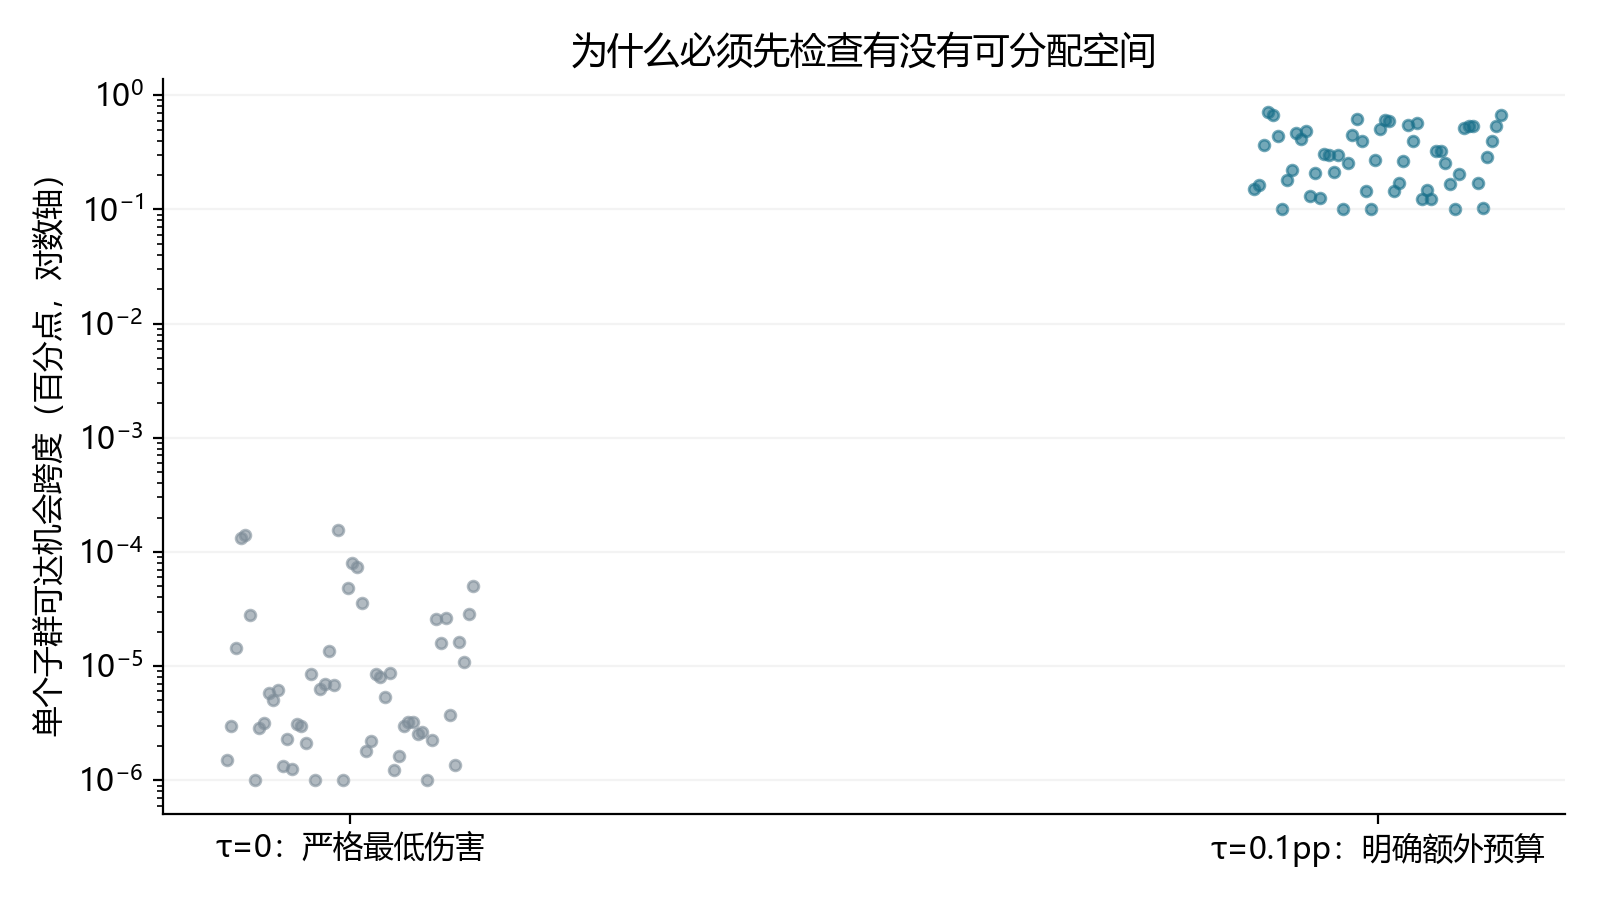
\includegraphics[width=.9\linewidth]{images/allocation_space.png}
\caption{业务可分配空间与数值退化。每种设置54个子群观测。}\end{figure}

\subsection{归一化分配是不同取舍，不是全面改进}
正预算下63条策略记录（9条收益基准、54条新分配规则）业务审计通过，18个完整 leximin 均通过归一化水位审计，无退化维度。所有18个配置中，完整 leximin 与一次归一化 maxmin 的实际结果在数值精度内相同；完整理论避免一般情况下的遗漏，但此次数据没有显示额外收益。

LightGBM 三种子测试均值如下，双预算均为1\%收益、0.1个百分点额外损害：
\begin{center}\small
\begin{tabular}{lrrrr}\toprule
方法 & 情景贡献 & 宏观差距pp & 最差误拒\% & 基准伤害D(pp)\\\midrule
旧绝对最弱组目标 & 35770.98 & 1.219 & 18.337 & 1.229\\
归一化机会目标 & 35786.89 & 1.475 & 18.548 & 1.155\\\bottomrule
\end{tabular}\end{center}
新目标贡献增加约15.91单位，最大附带损害降低约0.074个百分点，但最差群体误拒增加约0.211个百分点。更重要的是，单种子2pp宏观差距目标：新目标仅2/9个评分器满足，旧目标为5/9；LightGBM分别为1/3与3/3。均值不能掩盖个别配置超限。所有9个主配置的测试风险与收益底线仍满足。

因此不以归一化 leximin 直接替换已有主审批方法。它适合成为资源分配视角下的可解释对照，核心研究贡献进一步集中到双预算约束诊断与逆向机会价格。

\begin{figure}[htbp]\centering
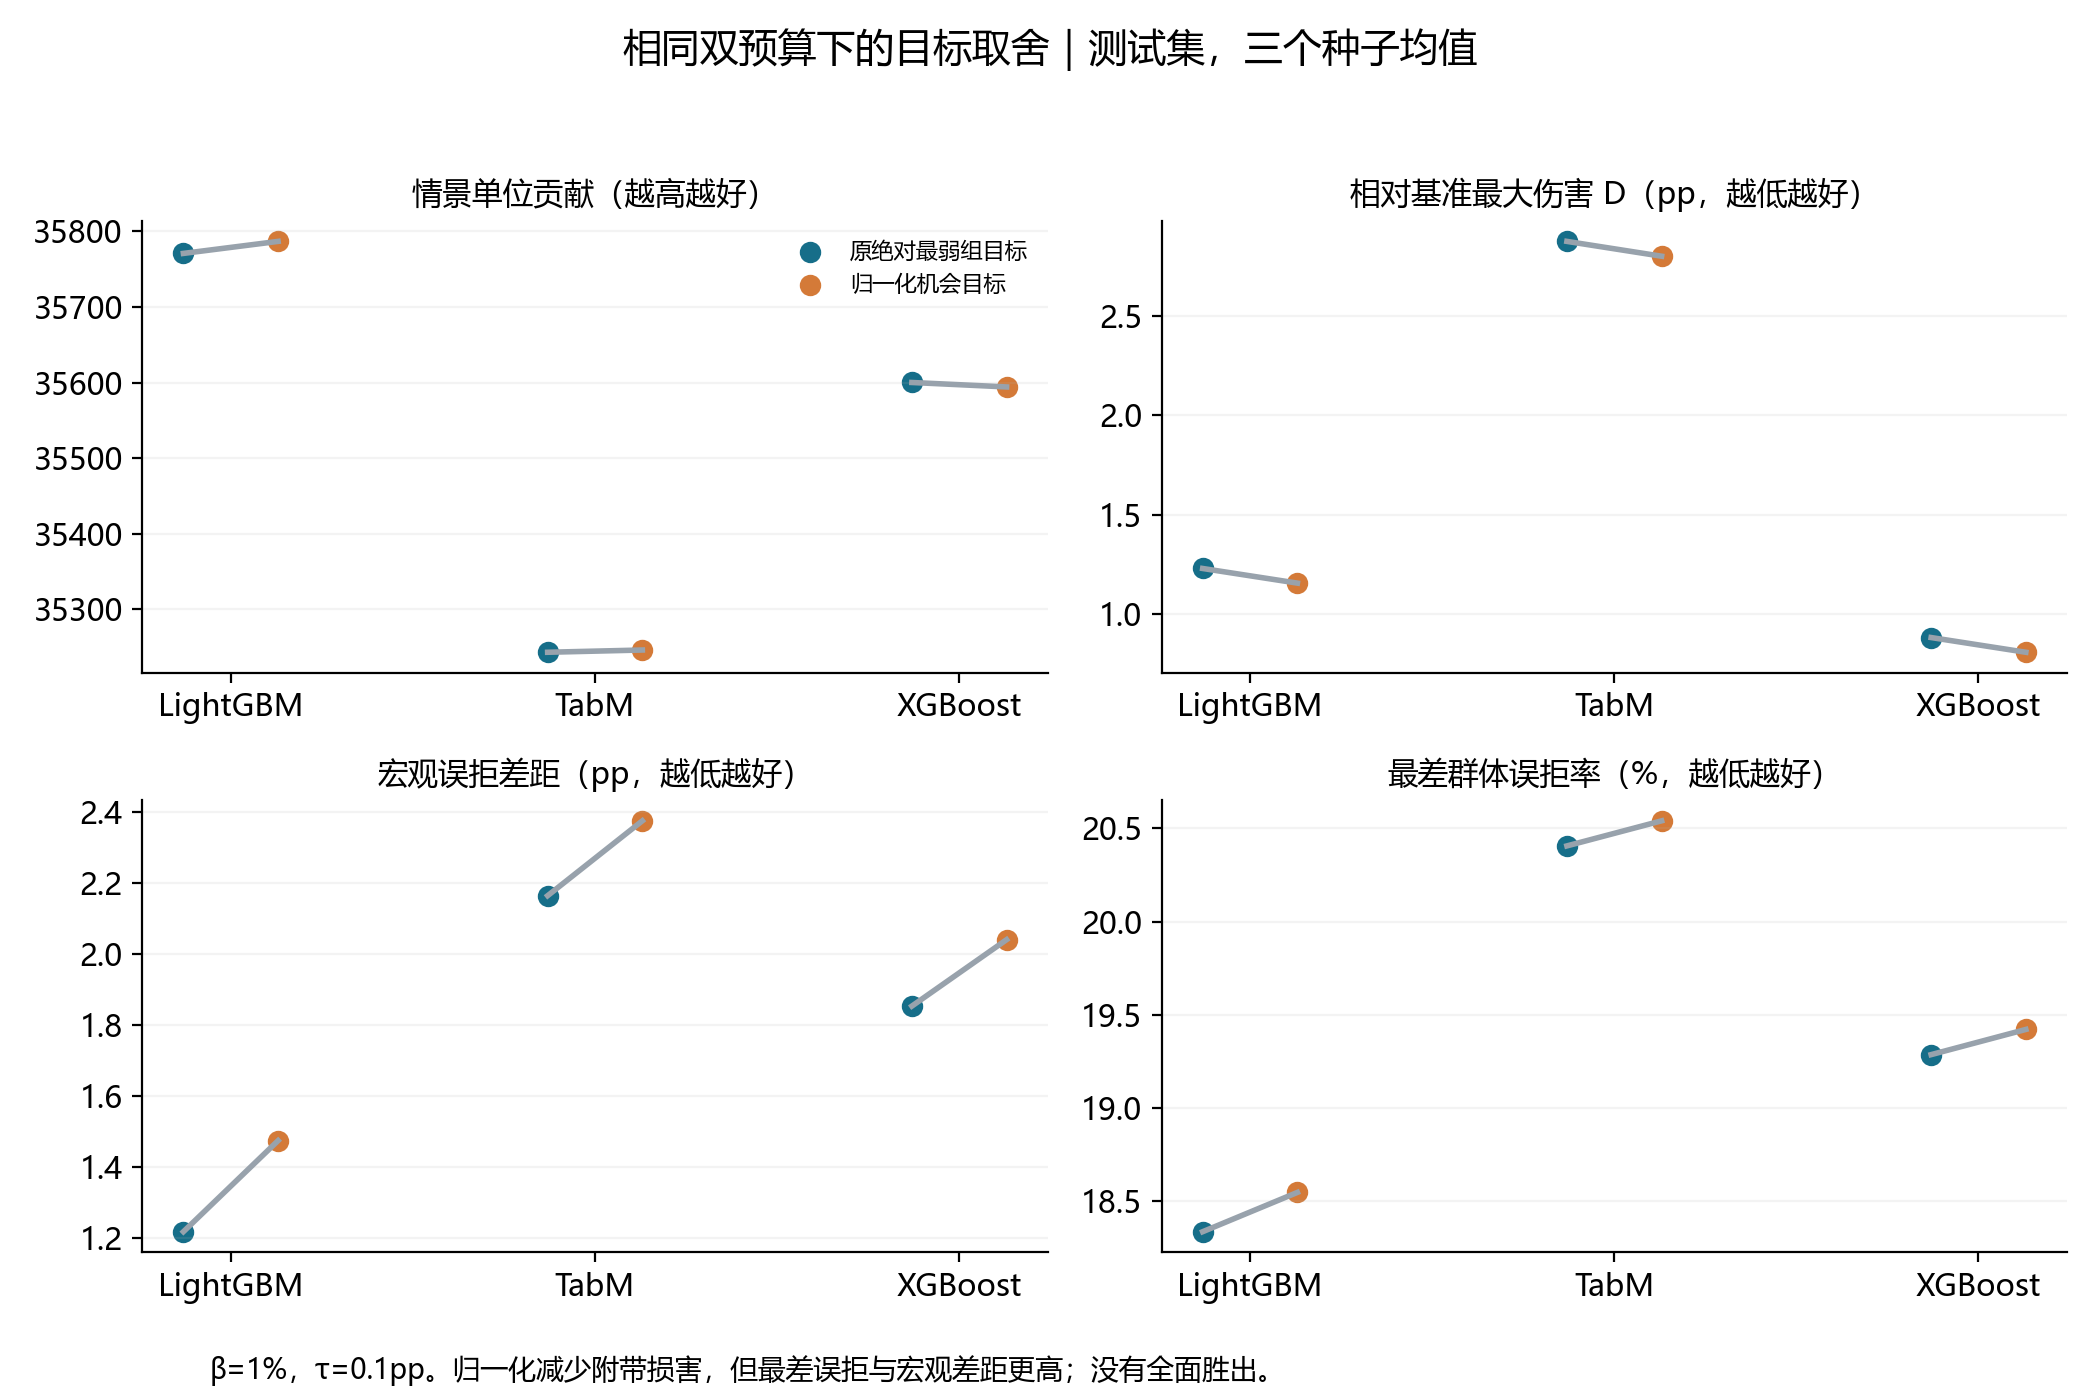
\includegraphics[width=\linewidth]{images/same_budget_tradeoff.png}
\caption{相同预算下三个模型的取舍，全部三个种子保留。}\end{figure}

\subsection{逆向机会定价：直接回应业务目标}
27个预设目标在验证集均可行，目标、风险、资金、收益及最低伤害价格均经重放检查。LightGBM三个种子的平均结果为：
\begin{center}
\begin{tabular}{rrr}\toprule
最弱机会底线提高pp & 最低额外伤害预算pp & 相对收益基准贡献变化\%\\\midrule
0.05 & 0.01589 & -0.1149\\
0.10 & 0.03643 & -0.1188\\
0.20 & 0.07753 & -0.1266\\
\bottomrule\end{tabular}\end{center}
这是最低保护价格，不是以人民币计价的利润损失；右列另报告情景贡献变化。每个目标的策略是在达到最低价格后再最大化贡献。均值之外，原始逐种子表与全部混合权重也已保存。

例如 LightGBM seed731：严格保护下最弱正常客户机会为80.119842\%，最低必要伤害为1.588621个百分点。要求共同机会底线提高0.10个百分点时，最低再允许0.022142个百分点额外伤害，得到相对收益基准约0.208968\%的贡献损失、5\%的风险。总损害上限约为1.610763个百分点，不应只报较小的额外部分。

\begin{figure}[htbp]\centering
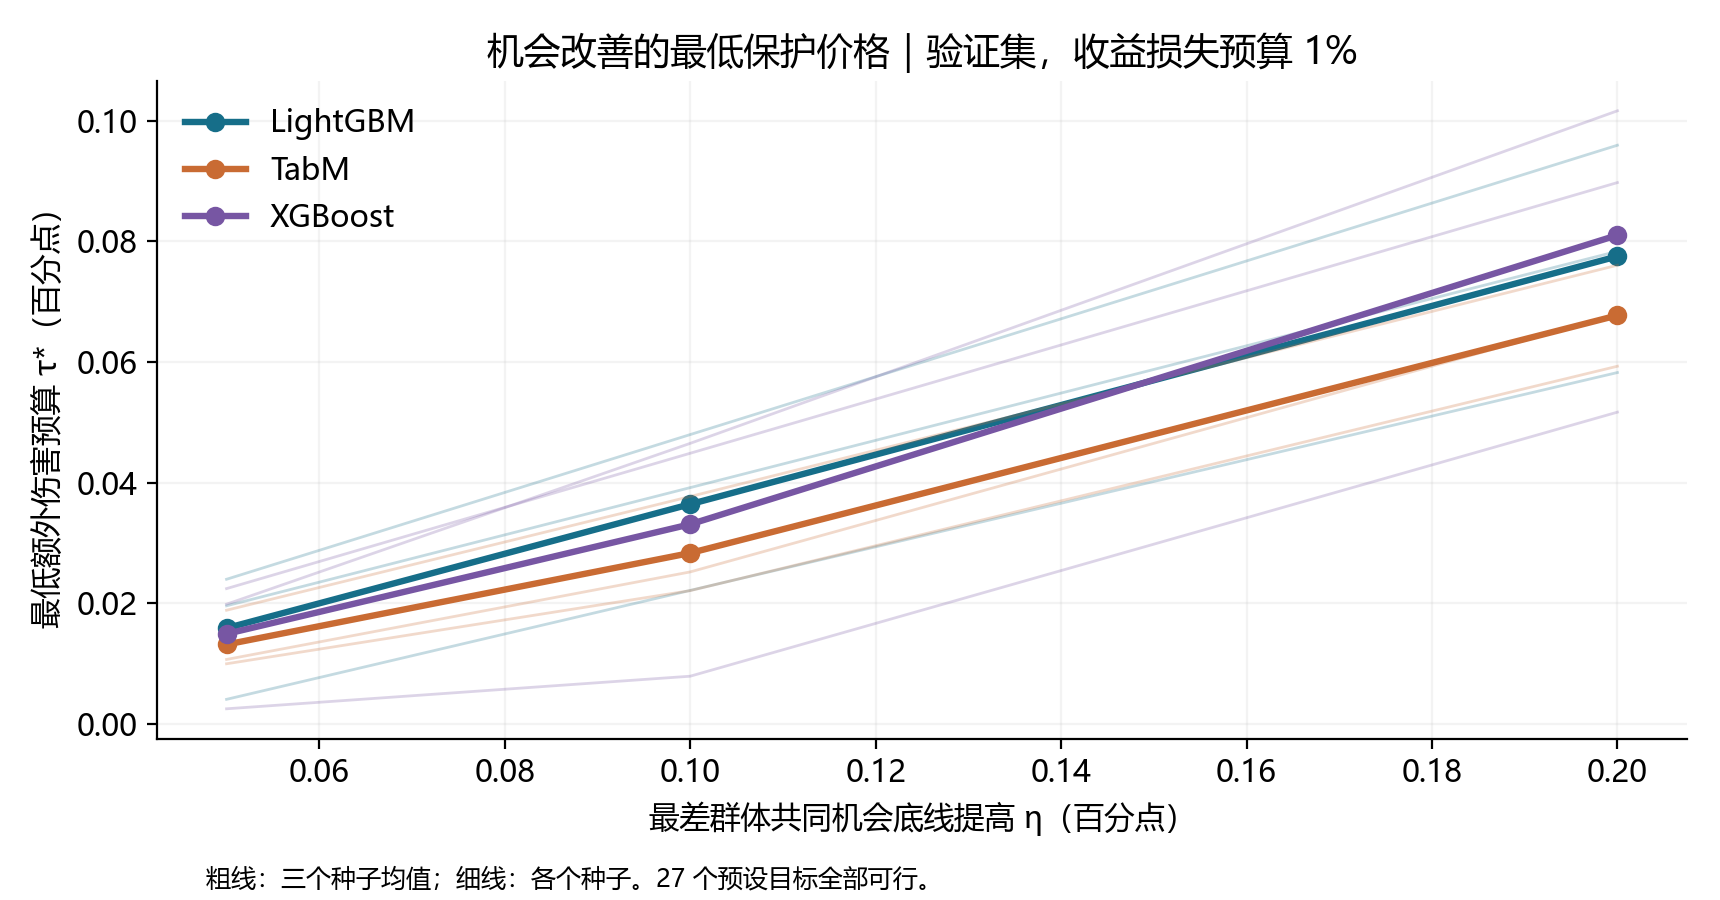
\includegraphics[width=.95\linewidth]{images/inverse_opportunity_price.png}
\caption{预设改善目标的最低额外保护价格。}\end{figure}

\subsection{冻结逆向定价策略的测试回放}
全部27个已保存策略随后在同一测试集重放，没有重新拟合或挑选目标。2160项独立检查通过；风险与收益底线27/27满足，2pp宏观差距仅8/27满足。相对各自冻结的严格保护W0策略，最差群体机会23/27提高，但只有9/27达到完整的预设提高幅度。因此，验证集逆向价格不能解释成未来样本的确定兑现保证。

LightGBM三个种子平均：预设提高0.05/0.10/0.20个百分点时，测试实际最差机会分别提高约0.0421/0.0922/0.1923个百分点。这里比较两个冻结策略在测试集上的最差机会之差，和验证集的绝对门槛 $W_0+\eta$ 区分记录。原始目标、未达标策略和收益变化全部保留在 \texttt{opportunity\_prices/test\_evaluation.csv}。

项目汇报应把双预算与逆向定价作为业务分析贡献，把原绝对最弱组方法继续作为当前表现较稳定的审批参考。这不依赖将新分配目标包装成全面性能升级。

\subsection{文件与复现}
实现位于 \texttt{research\_extension\_v3/theory\_extension}；本说明所在目录为 \texttt{theory\_note}。原始新结果位于 \texttt{results/run\_005\_theory} 与 \texttt{results/run\_006\_budget}，逆向定价位于后者的 \texttt{opportunity\_prices}。策略、配置、源代码快照或哈希、检查结果、配对区间、统计证书和原始图表均保留。原 run001--004 未改动。


\section{适合报告的研究主张}
我们不主张又训练出了一个领先所有方法的分类器。研究对象是同一组风险评分之上的审批决策：把“银行能损失多少”和“其他群体最多额外承担多少”分开建模；求出当前条件不可避免的伤害；借鉴资源分配决定有限机会如何分配；再把最弱群体改善转化为最低保护预算价格。精确问题的性质可以证明，数值实现与测试效果则分别验证。方法、逆向定价及保留的失败诊断共同组成项目证据。

\begin{thebibliography}{9}
\bibitem{drf}
Ghodsi et al. Dominant Resource Fairness: Fair Allocation of Multiple Resource Types. NSDI, 2011.
\url{https://www.usenix.org/conference/nsdi11/dominant-resource-fairness-fair-allocation-multiple-resource-types}
\bibitem{kelly}
Kelly, Maulloo, Tan. Rate control for communication networks: shadow prices, proportional fairness and stability. 1998.
\url{https://web.stanford.edu/class/cs244/papers/ShadowPricesFairnessStability.pdf}
\bibitem{lexfair}
Diana et al. Lexicographically Fair Learning: Algorithms and Generalization. FORC, 2021.
\url{https://drops.dagstuhl.de/entities/document/10.4230/LIPIcs.FORC.2021.6}
\bibitem{nash}
Zeng et al. Fairness-aware Meta-Learning via Nash Bargaining. NeurIPS, 2024.
\url{https://papers.nips.cc/paper_files/paper/2024/file/97a0f7d7fc2c26732943860241af1c7a-Paper-Conference.pdf}
\bibitem{massart}
Massart. The Tight Constant in the Dvoretzky--Kiefer--Wolfowitz Inequality. Annals of Probability, 18(3):1269--1283, 1990.
\url{https://doi.org/10.1214/aop/1176990746}
\end{thebibliography}
\end{document}